%\documentclass{article}
%\documentclass[handout]{beamer}
\documentclass{beamer}
%\usepackage{beamerarticle}
\usepackage{tikz}
\usetikzlibrary{arrows,shapes}

\author{S.Poss and A.Sailer}
\title{Luminosity spectrum measurement}
\subtitle{Update}

\mode<presentation>
{
   \setbeamertemplate{navigation symbols}{}
   \setbeamertemplate{footline}[frame number] 
}

\AtBeginSection[]
{
\begin{frame}<beamer>
\frametitle{Outline}
\tableofcontents[currentsection,currentsubsection]
\end{frame}
}


\begin{document}
\begin{frame}
\titlepage
\end{frame}
\begin{frame}
\frametitle{Outline}
\tableofcontents
% You might wish to add the option [pausesections]
\end{frame}
\tikzstyle{decision} = [diamond, draw, text badly centered, node distance=2.8cm]
\tikzstyle{block} = [rectangle, draw, text centered, rounded corners, text width=1.9cm, node distance=2.2cm]
\tikzstyle{autoblock} = [rectangle, draw, text centered, rounded corners, node distance=2.2cm]
\tikzstyle{line} = [draw, -triangle 90]
\tikzstyle{dline} = [draw, dashed, -triangle 90]
%\tikzstyle{cloud} = [draw, ellipse,fill=red!20, node distance=3cm,minimum height=2em]
\section{Introduction}

\begin{frame}
\frametitle{Introduction}
Last time:
\begin{itemize}
  \item Setup of model
  \item Study of pre-BHWide data (pre-Generator level)
\end{itemize}
Today:
\begin{itemize}
  \item BHWide data available
  \item Energy smearing 
\end{itemize}
\end{frame}

\section{Recap}
\begin{frame}
\frametitle{Last time's results}
Guinea Pig level fit to check the model
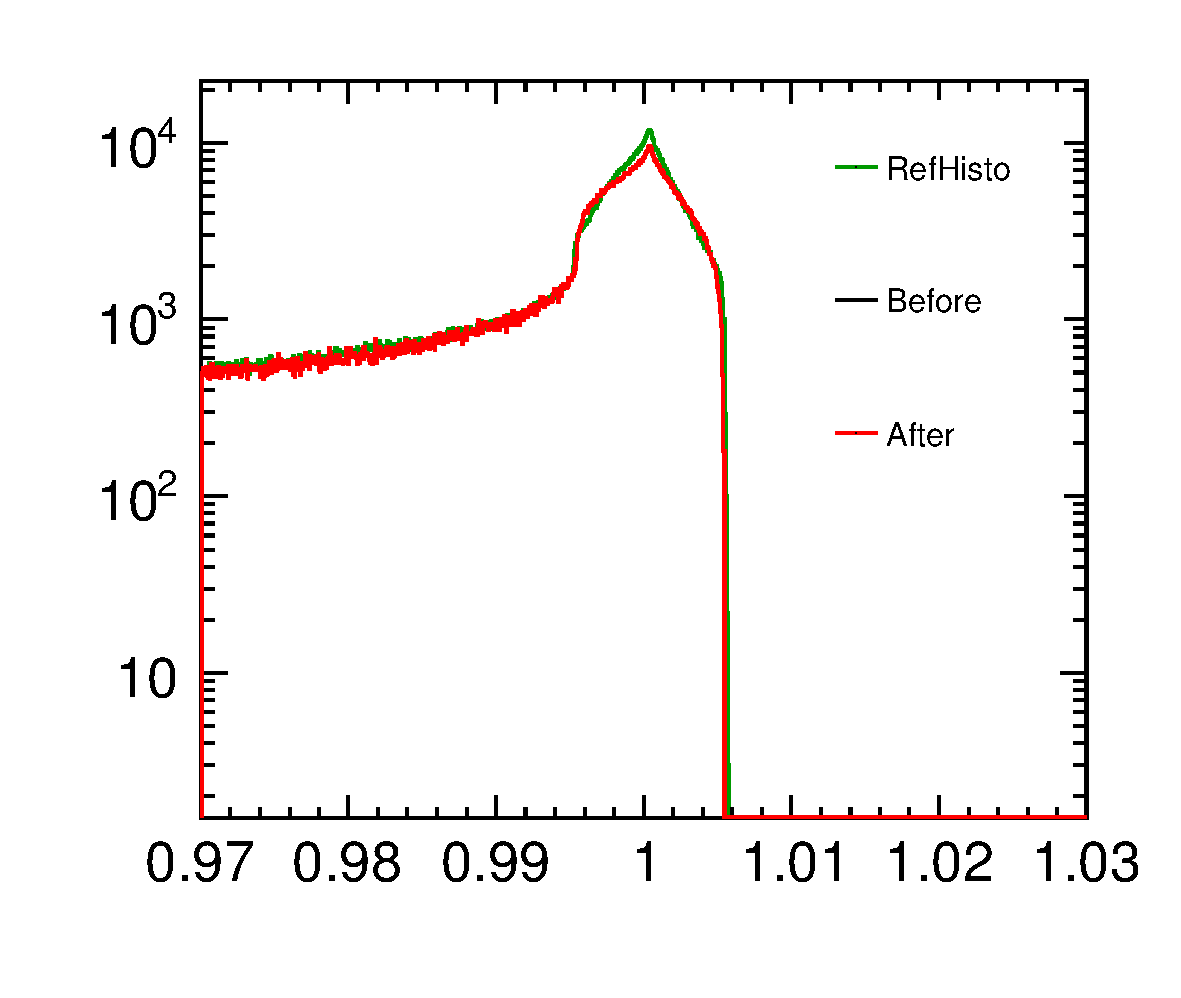
\includegraphics[width=9cm]{../HistoGrams}
\end{frame}

\section{Generating data: BHWide}
\begin{frame}
\frametitle{Generator: BHWide}
BHWide: The Monte Carlo Event Generator for Large-Angle Bhabha Scattering
\begin{itemize}
  \item Does not account for cross section dependency on $\sqrt{s}$ 
  (x-sec $\propto 1/s$): less events in the tails than in reality
  $\to$ less sensitivity in the tails (larger errors).
  \item Boost is applied after event generation.
  \item Produces electrons, positrons, and photons. \alert{Cut applied at
  generator level is  $7^\circ<\theta_{\textrm{leptons}}<173^\circ$}:
  xsec$=16\textrm{pb}$.
\end{itemize}
Cross section dependency can be corrected by generating more events in the tail before passing in BHWide.
Not done for today's analysis.
\end{frame}
\begin{frame}
\frametitle{Lepton distributions}
\includegraphics[width=9cm,page=7]{BHWideAnalysis.pdf}\\
Cut applied is done before boost treatement, thus the 13.8\%.
\end{frame}
\begin{frame}
\frametitle{Lepton distributions}
Effective C-M-E:
$\frac{\sqrt{s'}}{\sqrt{s}}=\sqrt{\frac{\sin\theta_1+\sin\theta_2+\sin(\theta_1+\theta_2)}{\sin\theta_1+\sin\theta_2-\sin(\theta_1+\theta_2)}}$\\
\includegraphics[width=9cm,page=8]{BHWideAnalysis.pdf}
\end{frame}
\begin{frame}
\frametitle{Photons}
\includegraphics[width=9cm,page=3]{BHWideAnalysis.pdf}
\end{frame}
\begin{frame}
\frametitle{Photons}
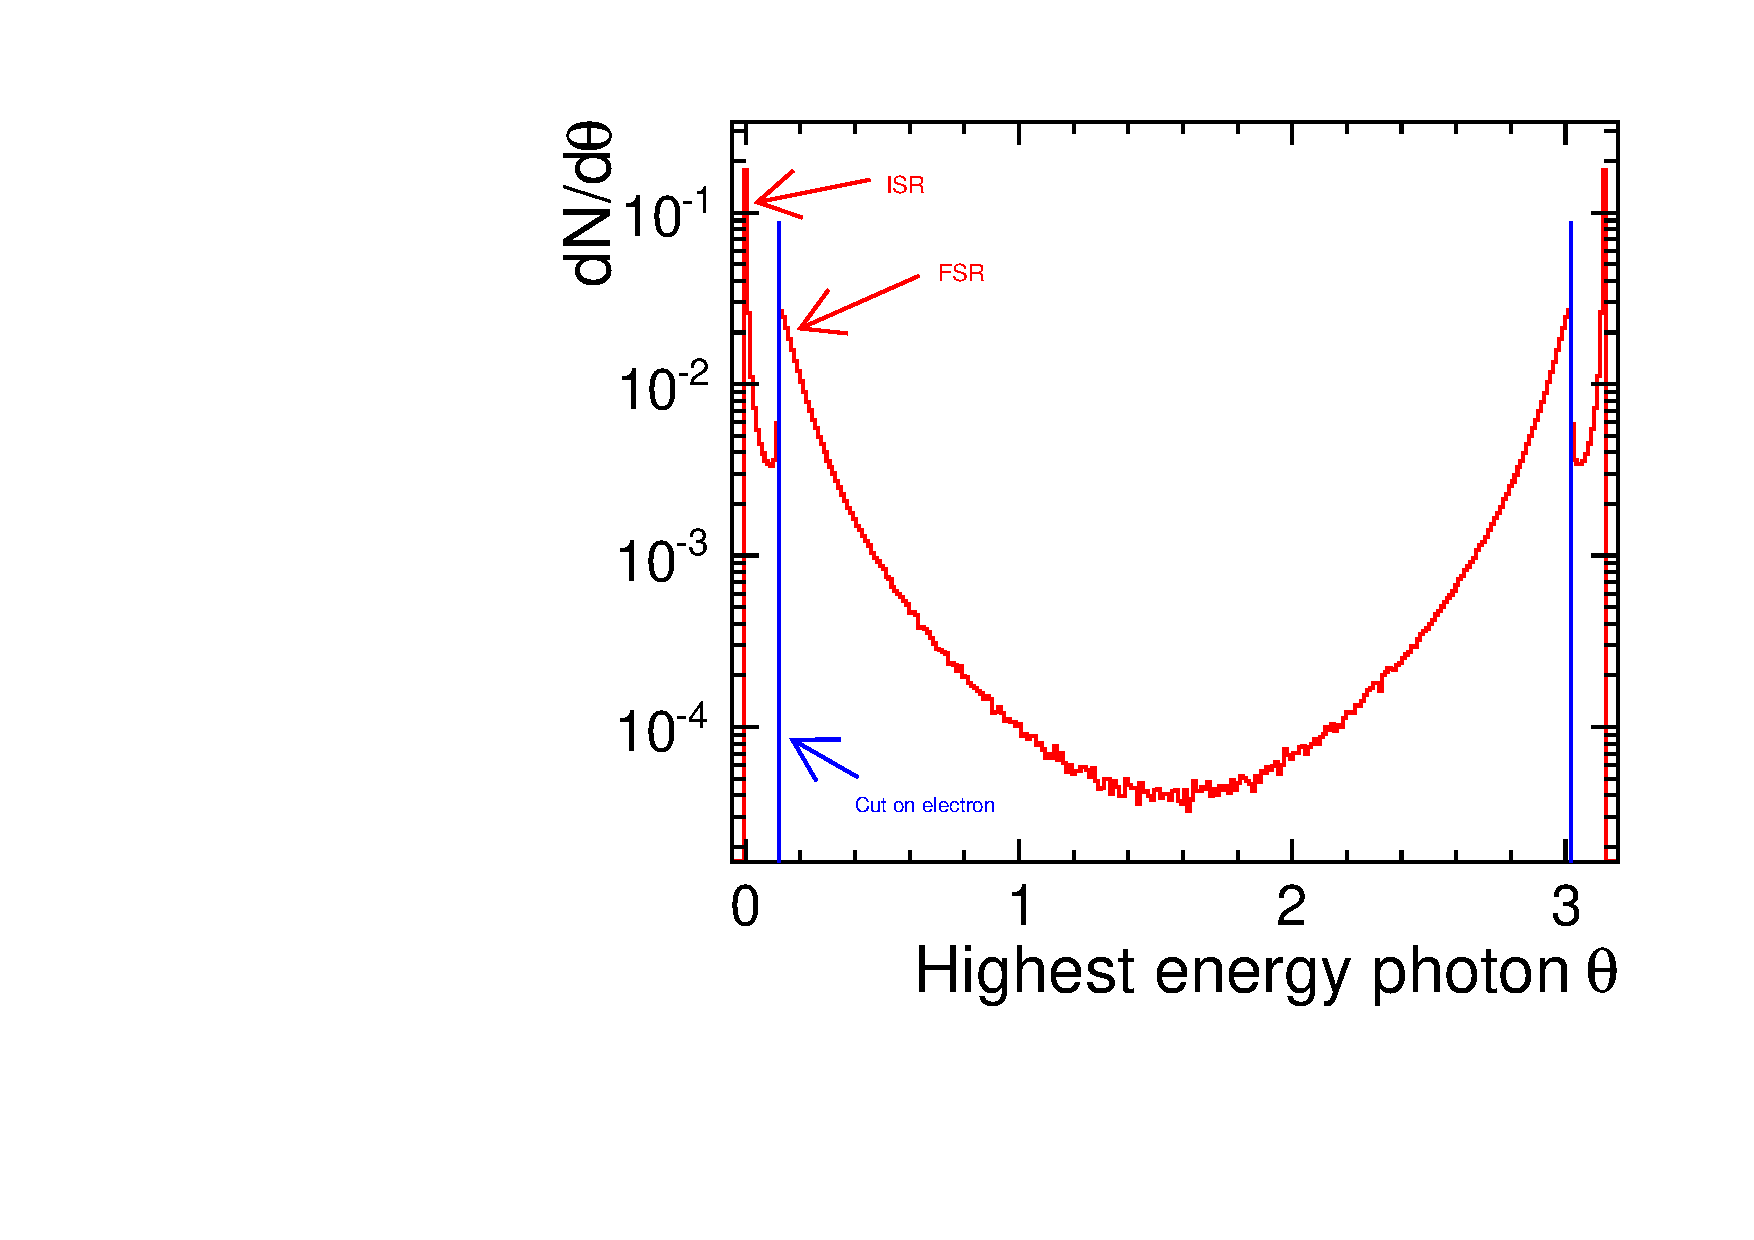
\includegraphics[width=9cm,page=1]{BHWideAnalysis.pdf}\\
BHWide generates photons from internal bremstrahlung (ISR and FSR).
\end{frame}
\begin{frame}
\frametitle{Photons}
Applying $7^\circ<\theta_{\textrm{photons}}<173^\circ$\\
\includegraphics[width=9cm,page=2]{BHWideAnalysis.pdf}
\end{frame}
\begin{frame}
\frametitle{Photon energy correction}
\includegraphics[width=9cm,page=5]{BHWideAnalysis.pdf}\\
Black line is $3^\circ$. This should be optimized on fully sim/reco data. 
\end{frame}
\begin{frame}
\frametitle{Photon energy correction}
Adding all photons' energy to the lepton if closer than $3^\circ$:\\
\includegraphics[width=9cm,page=6]{BHWideAnalysis.pdf}\\
Small effect on the energy.
\end{frame}
\begin{frame}
\frametitle{Generated statistics}
For the Guinea Pig sample: $5\times 10^6$ events.\\
For the Monte Carlo sample: $30\times 10^6$ events.
\end{frame}
\section{Energy smearing}
\begin{frame}
\frametitle{Energy smearing}
Why?
\begin{itemize}
  \item Because for the moment we do not have simulated data
  \item Because energy resolution is understood (CDR)
\end{itemize}
~\\
Which resolution function to use?
\begin{itemize}
  \item Pandora resolution (CDR): $\frac{\Delta p}{p} = a \oplus
  \frac{b}{p\sin\theta}$
  \item Ecal resolution (CDR): $\frac{\Delta E}{E} = \frac{15\%}{\sqrt{E}}$
\end{itemize}
In the very forward region (most of the events) the Pandora resolution is worse
than Ecal. \alert{Use Ecal resolution for the moment.}
\end{frame}
\begin{frame}
\frametitle{Energy smearing}
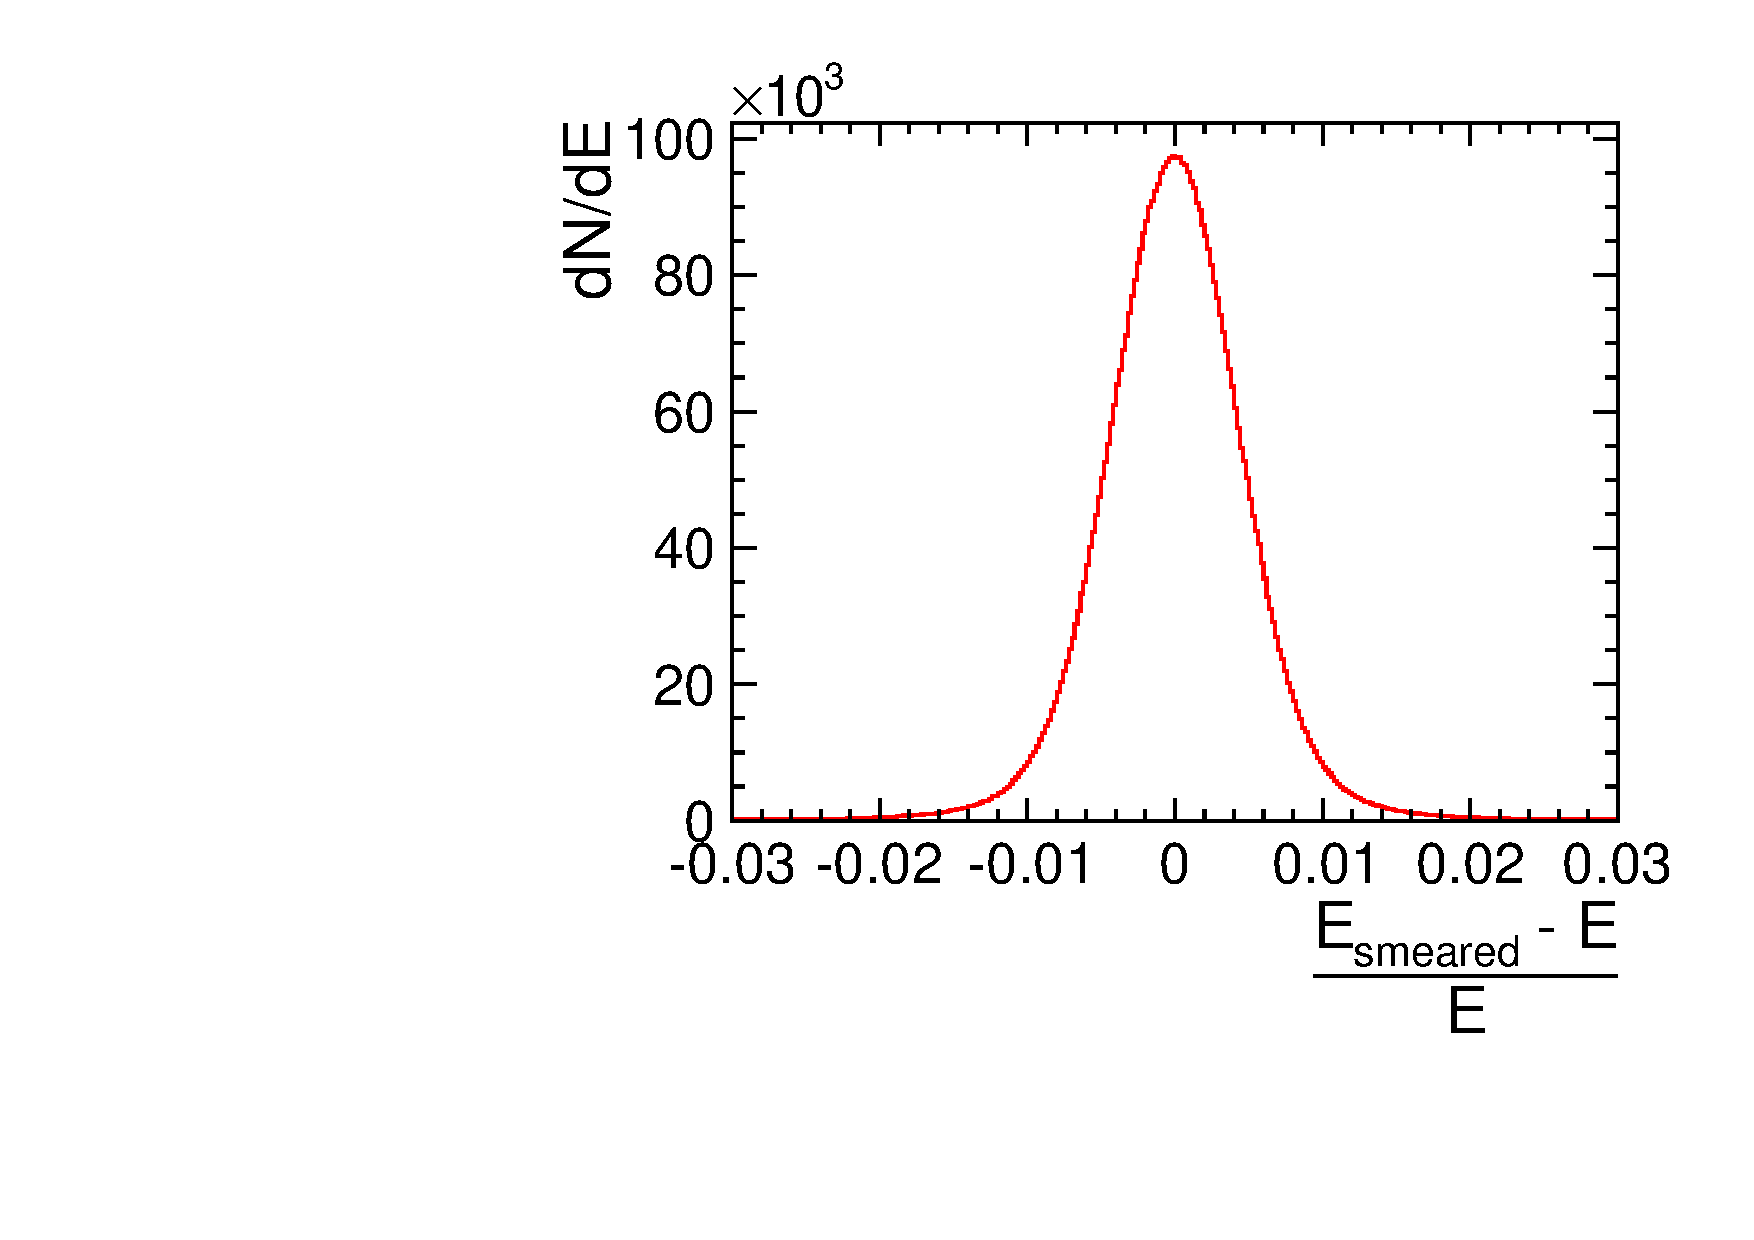
\includegraphics[width=9cm]{Smearing}
\end{frame}
\begin{frame}
\frametitle{Energy smearing}
\includegraphics[width=9cm,page=9]{BHWideAnalysis.pdf}
\end{frame}
\section{Angle smearing}
\begin{frame}
\frametitle{Angle smearing?}
None for the moment.
\end{frame}
\section{Fitting}
\begin{frame}
\frametitle{Fit update}
Pre-BHWide data 
\begin{itemize}
  \item 2D distribution (E beam1 and E beam2) to compute $\chi^2$
between MC and ``data''.
\item check our model
\end{itemize}
~\\
BHWide data (Generator level, smeared):
\begin{itemize}
  \item $E_{\ell1}$, $E_{\ell2}$, $\frac{\sqrt{s'}}{\sqrt{s}}$.
\end{itemize}
Those are ``reconstructible'' quantities, getting close to realistic situation.
$\frac{\sqrt{s'}}{\sqrt{s}}$ well measured from the angles.
\end{frame}
\begin{frame}
\frametitle{Fitting $3\times 10^5$ events ($\approx10$ days)}
Obtained 5 minutes before the meeting:
\begin{center}
\includegraphics[width=9cm,page=2]{final_res}
\end{center}
\end{frame}
\section{Conclusion}
\begin{frame}
\frametitle{Conclusion}
Small bug was found Friday, had to re-run everything. Correlation code is ready,
new plots to come.
\end{frame}

\end{document}
